\documentclass[a4paper,12pt]{article} 
% Paquetes......................................................................
\usepackage{amsmath, amssymb, amsfonts, latexsym}
\usepackage[utf8]{inputenc}
\usepackage[T1]{fontenc}
\usepackage{palatino}
\usepackage[full]{textcomp}
\usepackage{hyperref}
\usepackage{eurosym}
\usepackage[makeroom]{cancel}
\usepackage{array}
\usepackage{pdfpages}
\usepackage{float} % para que las figuras no floten

\textheight = 24 cm
\textwidth = 17 cm

\renewcommand{\arraystretch}{1.25}
\renewcommand{\contentsname}{Contenidos}


% INICIO DEL DOCUMENTO --------------------------------------------------------
\begin{document}
	
	\setlength{\parindent}{0.5cm}
	\setlength{\voffset}{-2cm}
	\setlength{\hoffset}{-2cm}
	
	\begin{center}
		\begin{LARGE}
			\textbf{Práctica Grupo 3}
		\end{LARGE}
		\begin{Large}
			\\ \medskip \text{Luis Couto Seller, Irene Marbán, Aída Muñoz Monjas}
		\end{Large}
		\rule{14cm}{0.5mm}
	\end{center}
	
	
	\tableofcontents
	
	\newpage
	\section*{Ejercicio 1}
	\addcontentsline{toc}{section}{Ejercicio 1}
	\textbf{Generación de números y variables aleatorias.} Describir el método \textit{Monty Phyton} para la distribución normal y compararlo con otros métodos para la
generación de valores de la normal.
	
	El objetivo del método Monty Python es lograr generar números aleatorios cuya frecuencia se aproxime a aquella de una distribución normal. 
	Para ello, emplea la similitud entre la función de densidad de una sigmoide decreciente y la función de densidad de la mitad de la distribución normal, de la manera que se indica en la imagen.
	
	\begin{figure}[H]
		\centering
		%% HACER FIGURA
		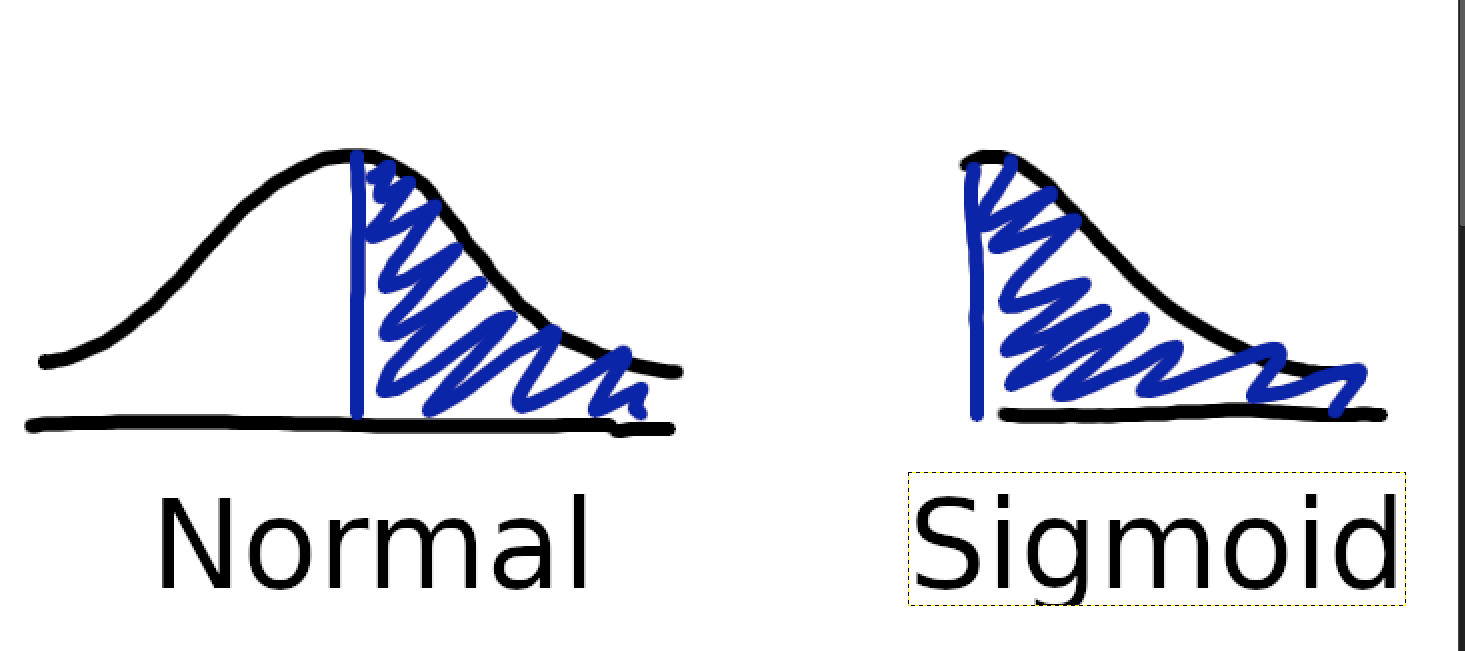
\includegraphics[width=0.65\textwidth]{include/normal_vs_sigmoid.png}
		\caption{Función normal (izquierda) frente a función de densidad de una sigmoide decreciente (derecha)}
	\end{figure}
	
	La función sigmoide utilizada es la descrita por $f(x)$ como se indica a continuación.
	$$f(x) = \dfrac{2}{\sqrt{2\pi}} \cdot e^{x^2/2} $$
	
	Tomando $x>0$, se traza un rectángulo de base $b$ y altura $1/b$ sobre la sigmoide. Realizando un giro de $\pi$ radianes y un desplazamiento sobre la región exterior al rectángulo, se pretende representar la mayor superficie posible de la sigmoide en el interior del rectángulo de área $1$. En las imágenes siguientes, podemos observar el procedimiento descrito tomando un $b=2.29$
	
	\begin{figure}[H]
		\centering
		%% HACER FIGURA
		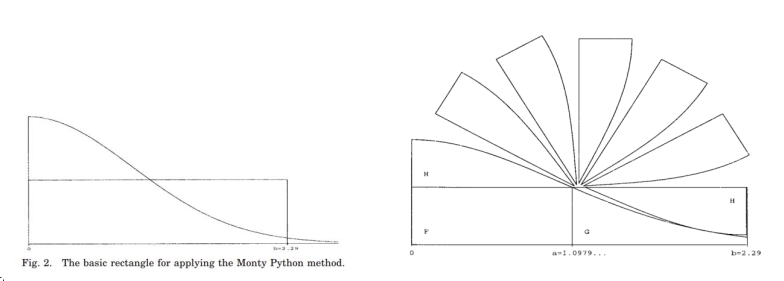
\includegraphics[width=0.9\textwidth]{include/rotating_sigmoid.png}
		\caption{Sigmoide con el rectángulo (izquierda), y descripción gráfica del giro descrito (derecha).}
	\end{figure}
	
	Una vez descrito el área bajo la función de densidad de la sigmoide en el interior del rectángulo, todo número aleatorio generado en ese rectángulo pertenecerá a las regiones $F$, $G$, $H$ o a la región comprendida entre $G$ y $H$ correspondiente a la cola de la sigmoide. La probabilidad de obtener un número en la cola es de un $0.022$.
	
	Entonces, siendo $(x,y)$ el valor aleatorio generado y $(x',y')$ su valor correspondiente en la sigmoide, se tiene
	$$
	(x',y') = 
	\begin{cases}
		(x,y) \quad \text{si} \quad x\in F \text{ ó } G \\
		(b-x,2/b-y) \quad \text{si} \quad x \in H
	\end{cases}
	$$  
	
	Si el valor aleatorio generado no pertenece a $F$, $G$ ó $H$, pertenecerá a la cola de la distribución, por lo que basta con devolver una variante de la cola normal mediante el método de Marsaglia o el método de la cola general de Marsaglia y Tsang.\\
		
	La elección del valor de $b$ no es crítica, pero elegir un valor de $b$ demasiado grande implica que habrá solapamiento al realizar el giro y desplazamiento descrito, mientras que si el valor de $b$ es demasiado pequeño, será necesario realizar frecuentemente el método para hallar los valores de la cola.
	En caso de utilizar el método anterior para "ajustar" la sigmoide al rectángulo, la elección de $b=2.29$ es prácticamente la máxima posible \cite{segundo-articulo}. \\
		
	En lugar de una rotación y un desplazamiento de la región exterior al rectángulo, "estirar" la región $H$ permite un ajuste mejor, manteniendo constante el área de la sigmoide, y por tanto siendo este un método más complejo pero más eficiente para realizar dicha aproximación. 
	
	Definiendo el factor de estiramiento $s$ y la función de densidad de la región $H$ $f_H(x)$ como 
	$$s=\dfrac{a}{b-a} \hspace{1.5cm} f_H(x)=f(x)-\dfrac{1}{b} \hspace{2mm} \text{con} \hspace{2mm} 0<x<a $$
	
	Por lo tanto, la región $H$ girada y estirada tiene una función de densidad
	$$ f_{H'}(x) = \dfrac{1}{b} - s  \left[ f(s (b-x) ) -\dfrac{1}{b} \right] $$ 
	La siguiente figura representa gráficamente las transformaciones matemáticas descritas compuestas con la rotación aplicada a la sección $H$. 
	
	\begin{figure}[H]
		\centering
		%% HACER FIGURA
		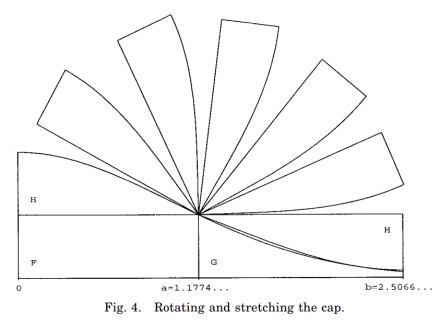
\includegraphics[width=0.5\textwidth]{include/stretching_sigmoid.png}
		\caption{Descripción gráfica del estiramiento descrito.}
	\end{figure}
	
	Para este segundo caso, la elección habitual para el valor de $b$ es $b= \sqrt{2\pi}$. Esta elección no es crítica, cualquier valor entre $2.506$ y $2.5074$ es válido \cite{segundo-articulo}, pero el par $b=\sqrt{2\pi}$, $a = \sqrt{\ln 4}$ son opciones fácilmente identificables con una precisión ilimitada.
	
	
	\newpage
	\section*{Ejercicio 2}
	\addcontentsline{toc}{section}{Ejercicio 2}
	\textbf{Simulación de sucesos discretos y optimización.}
	
	
	\newpage
	\section*{Bibliografía}
	\addcontentsline{toc}{section}{Bibliografía}
	\bibliography{include/references}
	\bibliographystyle{IEEEtran}
	
\end{document}